\section{System Model and Problem Formulation}
		\label{sec:model}
		
		
		
		\subsection{System Model}
		We consider a time-slotted system model in which the time horizon is divided to $T$ equal length slots ${t=\{1, 2, \dots ,T\}}$ (e.g., $T=24$ with time slots of $1$ hour length).
\subsubsection{Charging Network}
\label{sec:acn}
Our charging network model is inspired by the Caltech ACN~\cite{lee2018adaptive} as illustrated in Fig.~\ref{fig:model-a}. In \rev{the} Caltech EV charging network (located in a parking garage), electricity is distributed through a two-level transformer architecture from a main switch panel to multiple EV switch panels (\rev{$2$} panels in the current Caltech ACN). Each EV switch panel then is connected to several chargers ($\approx$25 chargers \rev{per panel} in the Caltech ACN). The total power drawn from the main switch panel \rev{by} the charging network has a power limit of  $p^\mathsf{total}$, that is determined by the facility operator to control the costs, reserve the capacity for other loads, and/or participate in demand-response programs.  
%This power, where we refer to it as \emph{network power limit} is used for both EV charging as well as non-EV charging purposes (e.g., lighting, fans, etc \cite{lee2018adaptive}). 
In other words, $p^\mathsf{total}$, which we refer to it as the \textit{global peak}, hereafter, limits the maximum aggregate EV charging load at each time slot. 
%The global peak must be less than or equal to the value obtained by subtracting non-EV load from network power limit. 
%When we write \emph{global peak constraint}, it refers to $p^\mathsf{total}$.  
%$p^\mathsf{total}$ is the maximum allowed aggregated electricity consumption by all stations at each slot and limits the total transferable power to EVs. 

We assume that there are $m$ EV switch panels that represent $m$ CSs. In addition to the global peak constraint, each CS $j$ has \rev{a} capacity constraint on \rev{its} total power drawn, indicated by $p_j$, and referred to it as the \emph{local peak} constraint. The \rev{value of} $p_j$ is determined by the output power limit of the transformers installed between the main switch panel and EV switch panels and could be different for each EV switch panel.  
%installed chargers in a CS have limited output power to charge EVs ~\cite{Wen,Xiang,Tesla}. Therefore, for CS $j$, $p_j$ cannot be more than sum of output power of its chargers. 
\rev{It is often observed that the charging demand of different CSs (EV switch panels in Fig.~\ref{fig:model-a}) are well below the local peak constraints.}
To reduce costs by taking advantage of flexibility due to heterogeneous charging demand of CSs, in the Caltech ACN, the global peak constraint of the main switch can be \textit{over-provisioned}, i.e., $p^\mathsf{total}$ is less than the aggregate local peaks,  ($\sum_j p_j\geq p^\mathsf{total}$). \rev{While this decreases costs, it also couples the problem of EV charging scheduling across different CSs.}
%Despite increased flexibility, the over-provisioning property, however, couples the problem of EV charging scheduling across different CSs. 
Our solutions in this paper will be centralized ones which can be obtained through communication between the CSs and a central server as illustrated in Fig. \ref{fig:model-b}.


%We make this clear by a simple example. Assume $m=2, p^\mathsf{total}=50$ kW and $p_1=p_2=25$ kW. In a specific time slot (e.g., $t=1$), the total demand in CS $1$ and $2$ is $40$ kWh and $10$ kWh, respectively. According to local peak constraints, it is not feasible to satisfy all demands in a single time slot. However, if we had $p_1=p2=50$ kW (e.g., by installing more chargers in the stations) we could be able to satisfy all demands by allocating $40 kW$ in $p_1$ and $10 kW$ in $p_2$ while still not violating $p^\mathsf{total}$. In case that $\sum_j p_j\leq p^\mathsf{total}$, the scheduling problem is not challenging and the solution can be obtained by solving the problem locally in each CS. If $\sum_j p_j> p^\mathsf{total}$ (which is the case we consider in this paper), a centralized solution is needed that can be obtained through communication between the CS and a central server as illustrated in Fig. \ref{fig:model-b}. 


\begin{figure}	
\centering
\minipage{0.49\textwidth}
				\begin{subfigure}[b]{0.69\textwidth}
					\begin{center}
						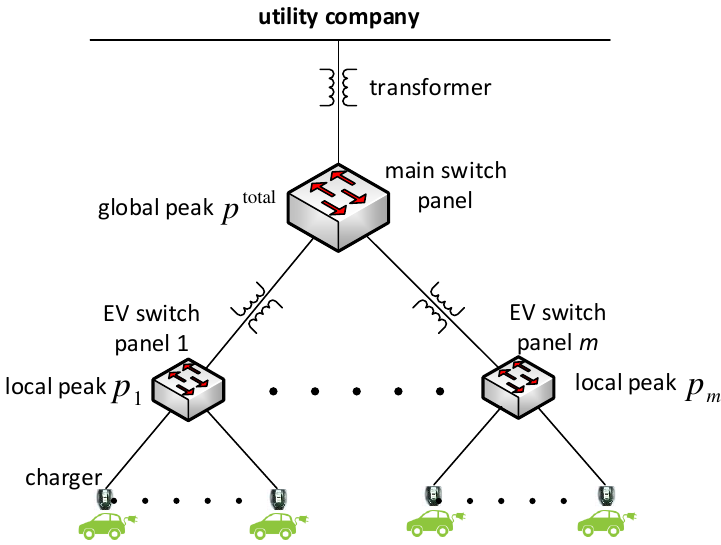
\includegraphics[width=\textwidth]{model-a.png}
						\caption{Caltech adaptive charging network (ACN)}
						\label{fig:model-a}
					\end{center}
				\end{subfigure}%
				\begin{subfigure}[b]{0.29\textwidth}
					\begin{center}
						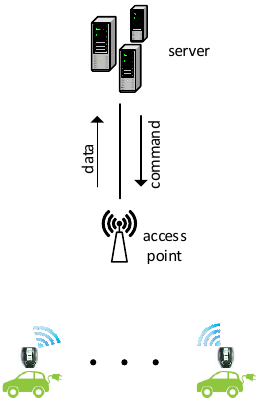
\includegraphics[width=\textwidth]{model-b.png}
						\caption{Communication model with server}
						\label{fig:model-b}
					\end{center}
				\end{subfigure}%  
\caption{System model \cite{lee2018adaptive}.} 
\label{fig:slackness1}
\endminipage
\end{figure}

		\begin{table} 
			\caption{Summary of key notations}
%			\vspace{-3mm}
			\label{tbl:not}
			\begin{center}
				\begin{tabular}{|c L{6.5cm}|}
					\hline
					\textbf{Notation} & \textbf{Description} \\
					\hline \hline			
					$T$ & Number of time slots, indexed by $t$\\			
					$m$ & Number of CSs, indexed by $j$\\			
					$n$ & Number of EVs, indexed by $i$\\			
					\hline
					\hline
					$a_i$ & Arrival time of EV $i$\\
					$d_i$ & Departure time of EV $i$\\
					$D_i$ & Demand of EV $i$\\
					$v_i$ & Valuation of EV $i$ for receiving its demand $D_i$ \\
					$k_i$ & Maximum charging rate of EV $i$\\
					$h(i)$ & CS of EV $i$\\
					\hline
					\hline
					$q_j$ & Maximum $k_i$ among all EVs in CS $j$\\
					$p_j$ & Maximum aggregate charging rate in station $j$\\
					$p^\mathsf{total}$ & Maximum aggregate charging rate of all stations\\
					\hline
					\hline
					$y_i^t$ & \textbf{opt. variable}, The amount that EV $i$ is charged at $t$ \\
					\hline
				\end{tabular}
			\end{center}
		\end{table}
		\subsubsection{EVs}
		\label{sec:ev} There are $n$ EVs in the system, indexed by $i$.
		%, all available at time $t=1$ to be charged\footnote{This assumption is reasonable for the %official buildings where the starting hour of the working day is fixed for all the %employers. Extensions to the case with different arrival times for the EVs, is part of the %future work.}. 
		EV $i$ is represented by a charging profile $\langle a_i,d_i,v_i,D_i,k_i\rangle$ 
		indicating its arrival time, departure time, willingness to pay, charging demand, and maximum charging rate, respectively. 
		%(depends on physical properties of EVs battery) 
		More specifically, the charging of EV $i$ can be scheduled within its \emph{availability window}, $[a_i,d_i]$. The charging rate at each slot is bounded by $k_i$, a parameter that depends on the physical constraints of the \rev{battery and on-board charger}. It is assumed that the charging profile of each EV is feasible with respect to its maximum charging rate and a slackness parameter $s\geq 1$, which is the minimum ratio between the park time of the EV and its minimum charging time, i.e., ${D_i\leq k_i(d_i-a_i+1)/s}$. The slackness parameter is imposed to tune the flexibility of the charging scheduling. In extreme case $s=1$,  the flexibility is minimum and the flexibility improves as $s$ increases. 
%		Note  that  the slackness  parameter  can  impact  the  total  revenue  and  is  investigated  in  simulation  experiments  in Section~\ref{sec:simul}.
		We assume that EV owners select their CS, perhaps the nearest to them, and so the assignments are given to the problem. Define $h(i)$ as the CS of EV~$i$.
		Moreover, $q_j$ denotes the maximum $k_i$ among all EVs in CS $j$, i.e., $q_j=\max_{h(i)=j} k_i$. 
		Finally, $v_i$ is the willingness to pay of EV $i$ to receive its entire demand $D_i$ before the departure time $d_i$. Note that in resource-constrained EV scheduling in ACN, it is not feasible to fulfill the entire demand of all EVs, hence, the problem turns into a resource allocation one with the goal of maximizing the aggregate value (a.k.a. utility) obtained from the EVs. In this way, each user can announce $v_i$ as its willingness to pay to get charged.
		%We assume that there is no gain for the CS if EV $i$ is partially charged. 
		
		% where $P$ defined as $P:\xi\rightarrow  \mathcal{P}$. 
\subsubsection{Revenue Models\label{sec:irm}} We consider two revenue models: 
\textit{(i) Fractional revenue model}: In this model, the fractional charging is allowed, i.e., the revenue from each EV is proportional to the fraction of the demand that is fulfilled \cite{Xiang} (see Eq.~\eqref{Eq:partial_value}). We tackle this model in Section~\ref{sec:fractional}.
\textit{(ii) Integral revenue model}: \rev{In this model, EV $i$ pays $v_i$ if it is fully charged and zero otherwise, i.e., there is no partial revenue for partial charging. }
%In this model, when EV $i$ is received its demand entirely, the gain is $v_{i}$ and zero, otherwise, i.e., there is no partial revenue for fractional charging. 
This is the model that is considered in~\cite{WTang,Shroff2014}. We tackle this model in Section~\ref{sec:integral}.
		
		%The actual aggregated peak of all parking stations must not exceeds global peak constraint. 
		
		
			\begin{table*}[!t]
			\centering
%	\vspace{-3mm}
			\caption{Proposed algorithms and their properties.}
			\label{tbl:algs}
			\begin{tabular}{ | l | c | c | c |c|}
				\hline
				\textbf{Algorithm} & \textbf{Revenue model} & \textbf{Type} & \textbf{Optimality} & \textbf{Complexity} \\ \hline\hline    
				\fcs& fractional& offline& Optimal & $O(n^2T+nT^2)$\\\hline 
				\ics& integral& offline& ${\Big( 1+\sum_{j=1}^m {\frac{p_j}{p_j-q_j}}.\frac{s}{s-1}\Big)}$-approximate & $O(nT\log T+n^2T)$ \\\hline 
				\focs & fractional& online& $2$-competitive & $O(n^2T)$\\\hline 
				\iocs& integral&  online& $b(1+\frac{p}{p-q}.\frac{s}{s-1})$-competitive, $(m=1)$ & $O(n^2T)$\\\hline
			\end{tabular}
		\end{table*}
		
		\subsection{Problem Formulation}
		\label{sec:problem}
	We formulate an optimization problem to schedule the charging of the EVs with the objective of maximizing total revenue obtained from charged EVs while respecting local and global peak constraints. 
		Note that each revenue model makes the underlying optimization problem fundamentally different. More specifically, the fractional charging model is a linear problem. 
		Integral revenue model, however, turns the underlying charging scheduling problem to a Mixed Integer Linear Program (MILP). The integer nature originates from the $0/1$-selection decision on EVs. 
%%%Recall that in integral revenue model the revenue is obtained given that the entire demand is fulfilled for the selected EV. 
		%We skip the explicit formulation of the problem under integral revenue model since it could be contemplated as the linear-relaxed version of the integral revenue model (for more explanation, we refer to the discussions in Section~\ref{sec:fractional}).
		We formulate  Scheduling Problem for Adaptive charging Network (\MCSP) under fractional revenue model as follows: 
		\bse
		\bee
		\MCSP: \max  && \sum\nolimits_{i=1}^n \frac{v_{i}}{D_i}\sum\nolimits_{t=a_i}^{d_i} y_i^t \label{Pobjec} \nonumber\\
		\text{s.t.} &&\sum\nolimits_{t=a_i}^{d_i} y_i^t\leq D_i,\quad\quad\forall i, \label{ConstPartial} \\
		&&  \sum\nolimits_{i=1}^n y_i^t\leq p^\mathsf{total} ,\quad\quad\forall t,\label{ConstTotal} \\
		&&\sum\nolimits_{i:h(i)=j} y_i^t\leq p_j ,\quad\quad\forall t,j,\label{ConstLocal}\\
		&& y_i^t  \leq \frac{k_i}{D_i}\sum\nolimits_{t^\prime=a_i}^{d_i} y_i^{t^\prime}, \quad\forall i,t,\label{ConstSpeed}\\
%		&& \rev{y_i^t=0,\forall t\in\{t':t'>d_i \vee t'<a_i\}}, \\
		\text{vars.} && y_i^t \geq 0, \quad\quad\forall i, t,\label{ConstPositive}\nonumber
		%&& s_v(t), \quad \forall v,t
		\eee
		\ese
		where $y_i^t$ is the amount that EV $i$ is charged at slot $t$. Constraint (\ref{ConstPartial}) ensures that the aggregate amount received by EV $i$ is at most the demand $D_i$. 
%		Note that under integral revenue model, when we design our algorithm, we do not allow partial charging. 
The global and local peak constraints are represented by constraints (\ref{ConstTotal}) and (\ref{ConstLocal}), respectively. 
		
		\revv{The constraint~\eqref{ConstSpeed} enforces the maximum charging rate of EVs. The straightforward way to express this constraint is to simply state that at each time slot $t$, the charging rate of EV $i$ should be less than or equal to its maximum charging rate, i.e., $y_i^t\leq k_i, \forall i,t$. 
		However, for the sake of effective algorithm design for integral model and reducing the integrality gap of the relaxed linear problem, this constraint is strengthened in the form of Eq.~\eqref{ConstSpeed}. 
		Note that in case that the aggregated charging of EV $i$ during its availability window is equal to its demand, i.e., $\sum_{t^\prime=a_i}^{d_i} y_i^{t^\prime}= D_i$, Eq.~\eqref{ConstSpeed} reduces to the simple form of $y_i^t\leq k_i$.  
		This is a natural way in approximation algorithm design to improve the performance of the algorithms under linear-relaxation based design~\cite{Carr}. } 
	
	
The \MCSP is an extension of formulated problem in \cite{Jain} where a job scheduling problem in cloud applications is studied. It turns out that the resource allocation problem in cloud systems and the EV charging scheduling problem in a \emph{single station} share similar structure. Indeed, each charging profile in our scheduling problem can be seen as a job in cloud system with a deadline, value, and CPU demand. The \MCSP, however, comes with an additional constraint~\eqref{ConstTotal}, which makes it different from the problem in \cite{Jain}, such that the existing solution \revv{will not} work in the new setting. More importantly, this paper studies both offline and online solutions for the problem in both fractional and integral settings, while \cite{Jain} tackles only the offline integral model.  
		
%(ii) Our solution design and analysis for integral revenue model is based on linear-relaxation primal-dual framework~\cite{Jain}. Therefore, in Section \ref{sec:integral} for integral revenue model, we rely on the \MCSP for the analysis of the proposed algorithms and skip to explicitly formulate the original MILP problem.



%		Also, we cover the fractional revenue model and provide theoretical bounds for the proposed algorithms.
		
%In the next two sections, we devise several algorithms to solve the \MCSP under the two revenue models (integral and fractional) and for both offline and online scenarios. 
